\newpage

\section{RESULTADOS}

\hspace*{0.8cm} Neste capítulo são abordados os resultados obtidos durante o desenvolvimento do trabalho de conclusão de curso. Destaca-se neste projeto dois resultados significativos, um deles é o protótipo físico desenvolvido, apresentado na Figura \ref{fig:mama} e o outro resultado diz respeito as formas de ondas obtidas que compõe mo sinal de ECG, formando pela onda P, complexo QRS e onda T. \textcolor{red}{E O BAIXO CUSTO????}

Os componentes utilizados na montagem do protótipo são apresentados no capítulo 3. Após, as etapas de montagem, soldagem e configuração, realizou o acomodamento do sistema, para isso utilizou uma caixa patola deixando apenas um espaço destinado conexão do cabo-flat com os pinos do Raspberry e a entrada do cabo paiciente, destaca-se que esse tipo de caixa é amplamente utilizada para acabamento estético, proteção de circuitos. A Figura \ref{fig:mama}, representa o dispositivo final, disposto na caixa patola.




\begin{figure}[H]
\begin{center}
			\caption{Dispositivo final, disposto na caixa patola}
			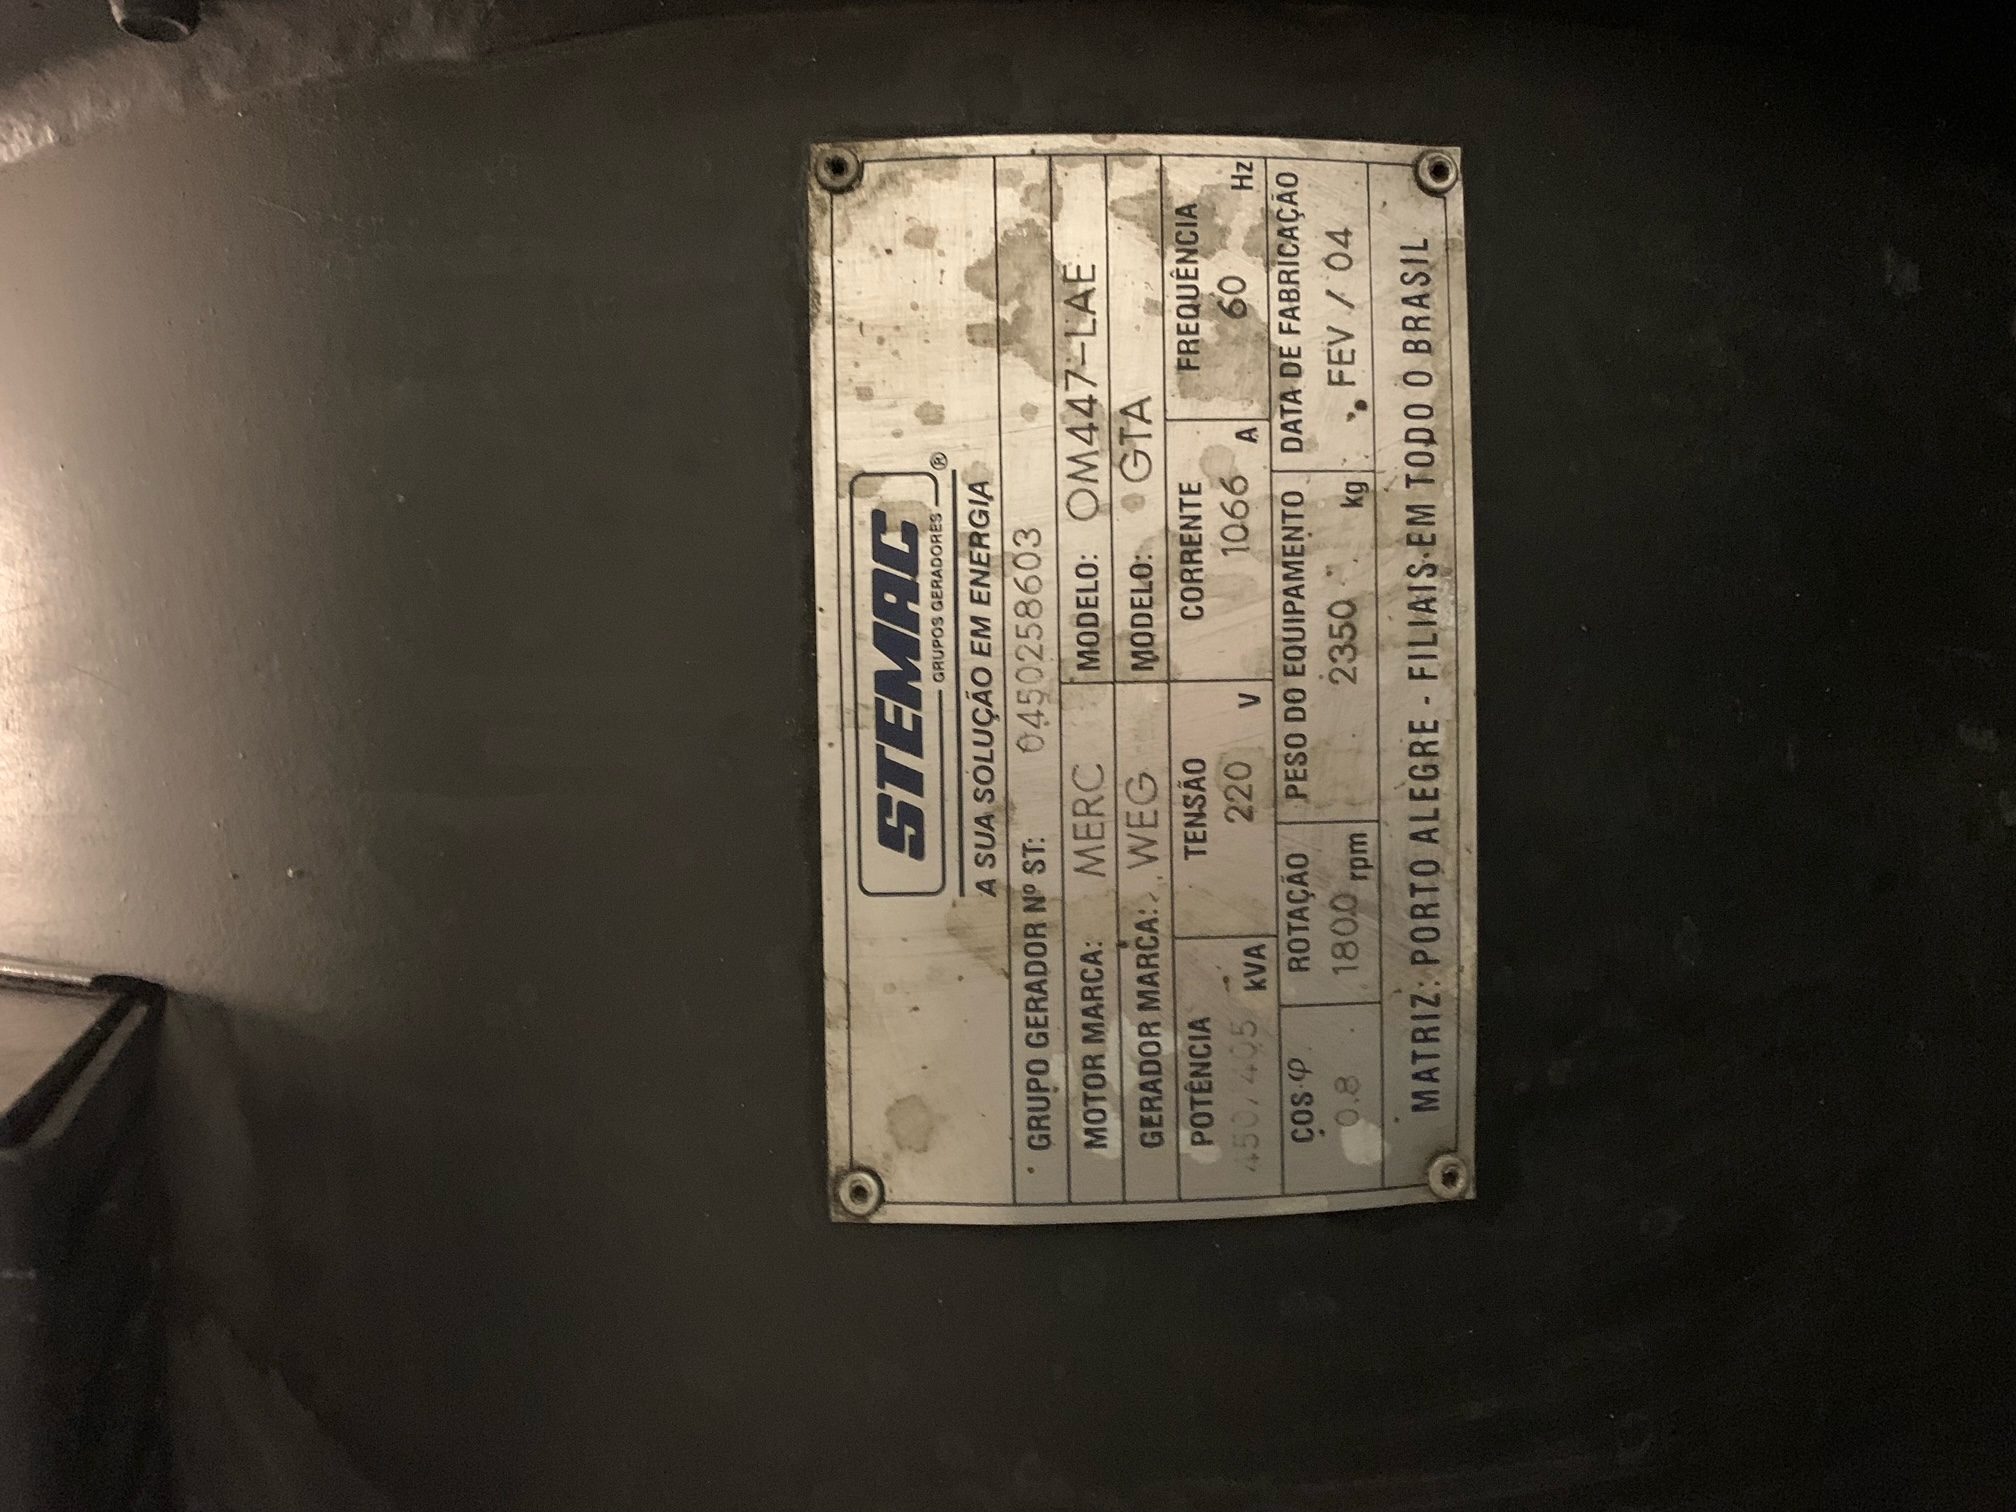
\includegraphics[width=.9\textwidth]{Figuras/info_gerador_450.jpeg}
              \vspace*{\fill} 
            \begin{quote} 
            \centering 
           Fonte: Elaborada pela autora
            \end{quote}
            \vspace*{\fill}
			
			\label{fig:mama}
\end{center}
\end{figure}
A utilização da placa baseada no CI AD8232 da Analog Device para obtenção dos sinais de ECG foi importante para eliminar as variáveis do processo de aquisição. O protótipo desenvolvido foi testado com o simulador de sinais vitais HS-15, e seus resultados foram comparados aos resultados da forma de onda padrão da segunda derivação eletrocardiográfica de um equipamento comercial modelo EP-12 da empresa Philips Dixtal \textcolor{red}{AQUI VAI UMA REF}.

A Figura \ref{fig:popi}, representa o sinal ECG simulado no equipamento eletrocardiógrafo EP12, o equipamente utiliza o mesmo modelo de simulador de sinais vitais utilizando neste trabalho. É possivel, analisar e verificar a semelhança com a o sinal exposto na Figura  \ref{fig:oscilo}.  O propósito deste projeto é fornecer com qualidade e parâmetros as formas de ondas característica do ECG. \textcolor{red}{MELHORE ESSA ULTIMA FRASE}

\begin{figure}[H]
\begin{center}
			\caption{Sinal de ECG simulado no EP12 Dixtal}
			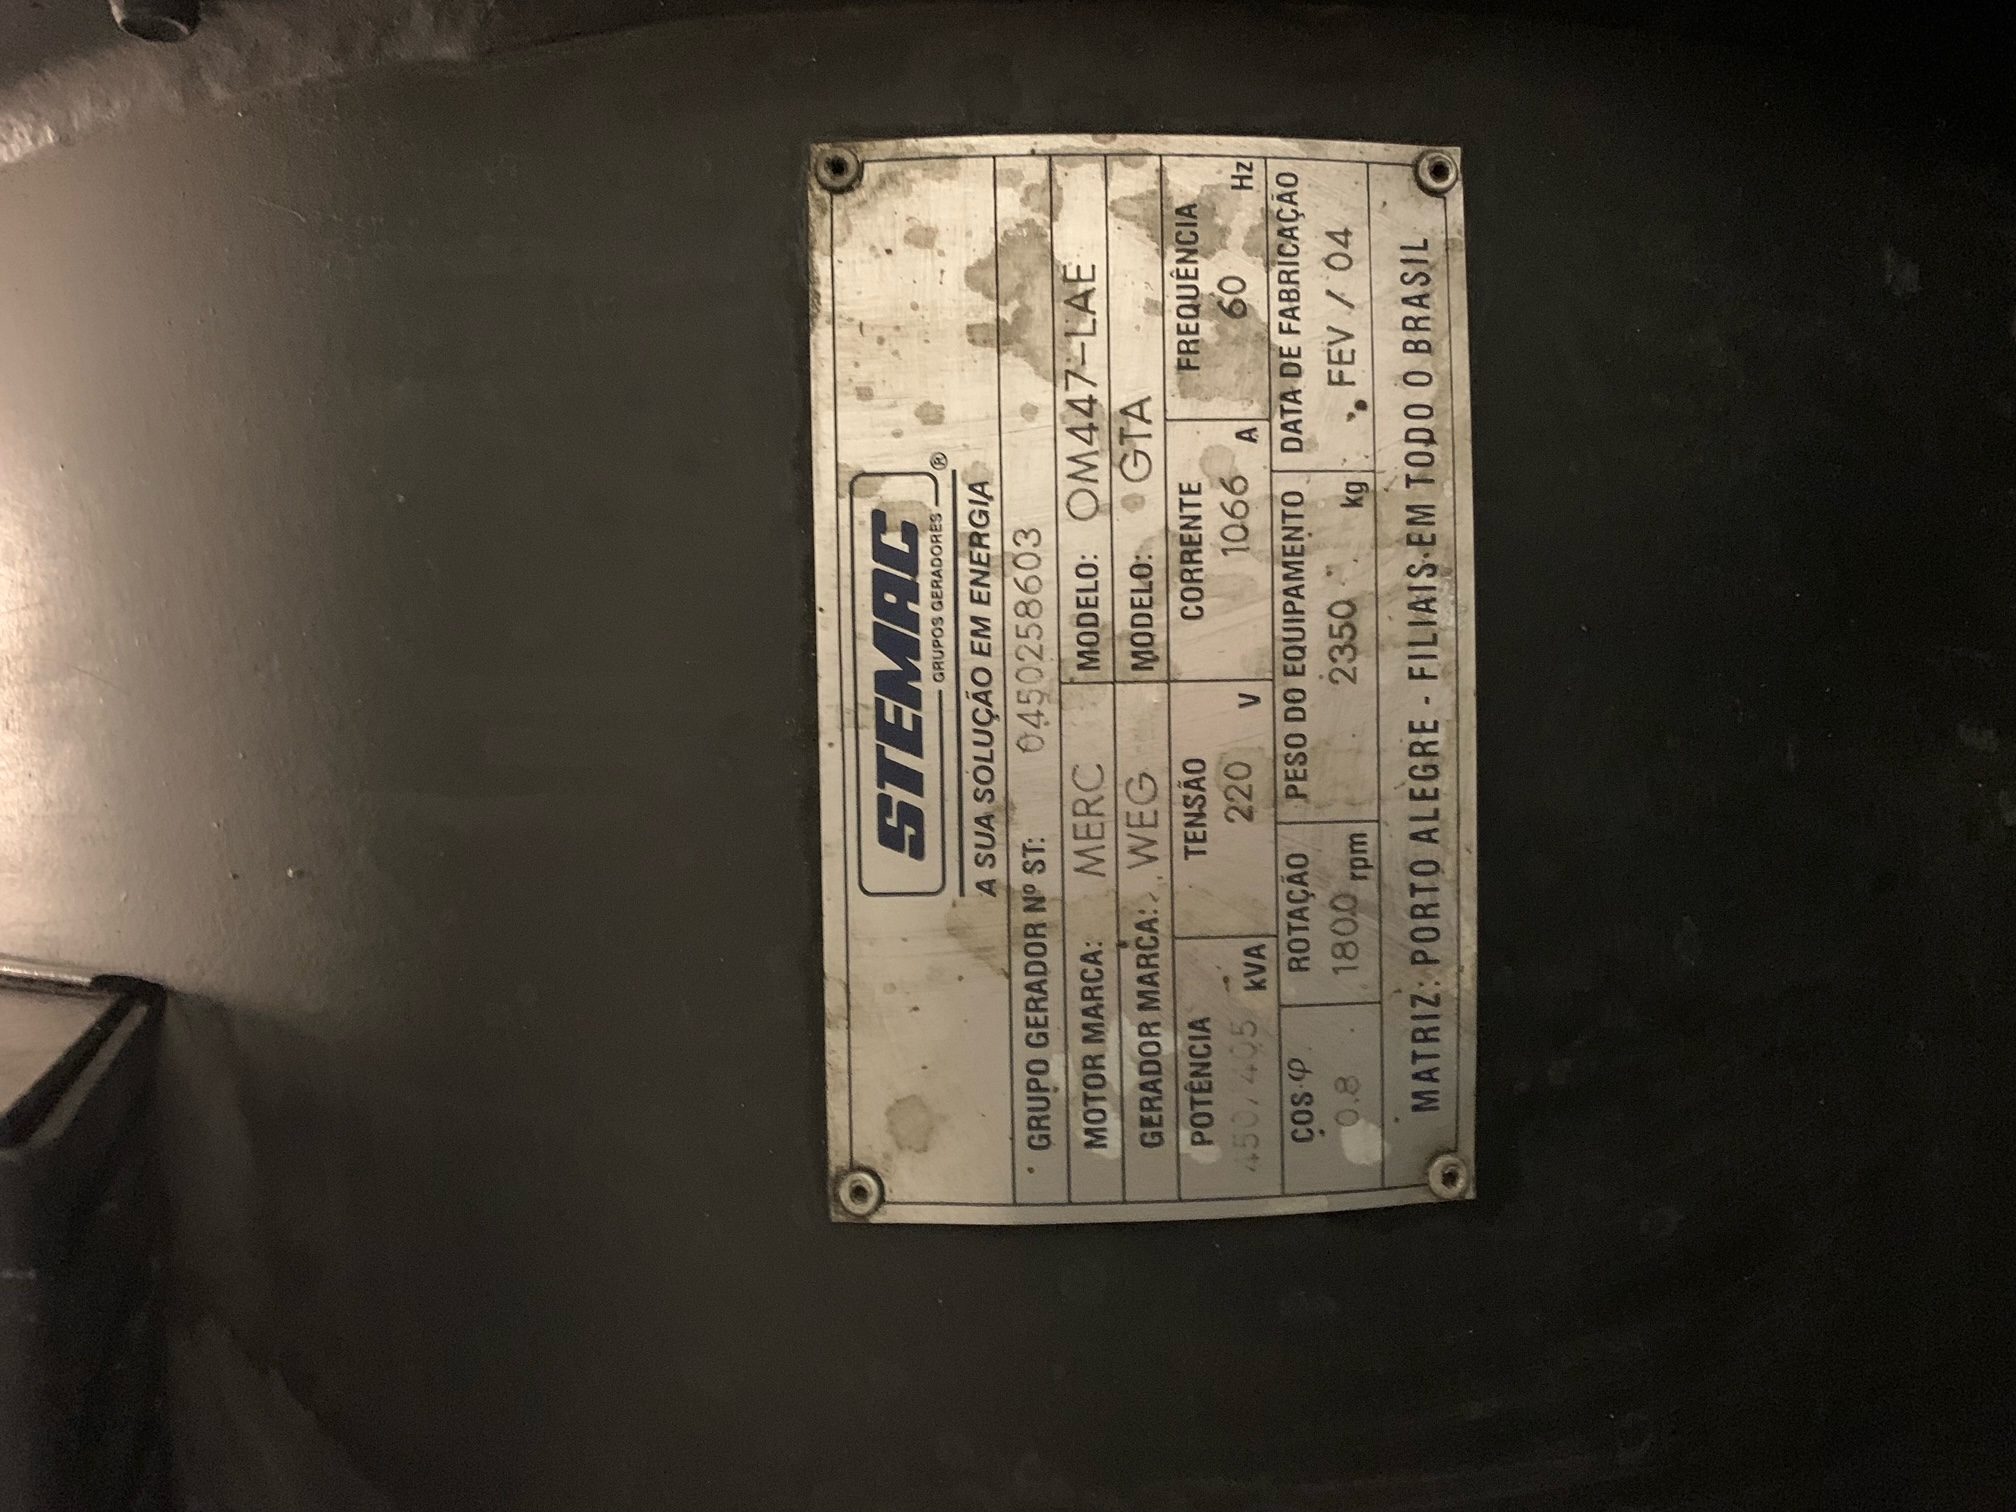
\includegraphics[width=.8\textwidth]{Figuras/info_gerador_450.jpeg}
              \vspace*{\fill} 
            \begin{quote} 
            \centering 
           Fonte: \cite{ronald}
            \end{quote}
            \vspace*{\fill}
			\label{fig:popi}
\end{center}
\end{figure}

A Figura \ref{fig:oscilo}, representa a forma de onda adquirida pelo o sistema de aquisição, utilizando o simulador para gerar sinais vitais e o oscilóscopio para análise. Este sinal é composto pela a onda p, complexo QRS e a onda T, característico da forma de onda do eletrocardiograma. \textcolor{red}{MELHORE ESSE PARA...ESCREVA MAIS OU MENOS ASSIM: NA FIGURA TAL, APRESENTA-SE A FORMA DE ONDA....SACOU??...EM GERAL, PROCURE ESCREVER ASSIM...OU SEJA, CORRIJA O RESTO...}

\begin{figure}[H]
\begin{center}
			\caption{Sinal do ECG obtido pelo o osciloscópio}
			\includegraphics[width=.9\textwidth]{Figuras/oscil.PNG}
             \vspace*{\fill} 
            \begin{quote} 
            \centering 
           Fonte: Elaborada pela autora
            \end{quote}
            \vspace*{\fill}
			\label{fig:oscilo}
\end{center}
\end{figure}

\hspace*{0.8cm}O Raspberry Pi 3 está sendo usado como servidor. O cliente solicita através do comando 'req' e para cada amostra é determinado um valor de acordo com o sinal fornecido pelo o simulador através da porta do mcp.read-adc(4), ou seja, a porta 4 do conversão analogico/digital. Essa leitura está sendo comprovado na Figura \ref{fig:kiki}.

\begin{figure}[H]
\begin{center}
			\caption{Amostragem Sinal do ECG}
			\includegraphics[width=.9\textwidth]{Figuras/json.PNG}
			              						\vspace*{\fill} 
            \begin{quote} 
            \centering 
           Fonte: Elaborada pela autora
            \end{quote}
            \vspace*{\fill}
			\label{fig:kiki}
\end{center}
\end{figure}

Os testes de transmissão e recepção do sinal utilizando a arquitetura cliente-servidor proposta foram realizados conectando os dispositivos através da rede Wi-fi do HUB. Com o resultado dessa arquitetura, tem-se a forma de onda utilizando o simulador de sinais vitais, conectado ao protótipo. Nestes testes, utilizou-se o simulador e foi variado a amplitude e o batimento por minuto.

A Figura \ref{fig:ecg2}, representa um resultado da arquitetura e o protótipo. A imagem representa o sinal ECG simulado, composto por 500 amostras de amplitude do sinal em determinado tempo. Esse sinal é composto inicialmente pela a onda P, complexo QRS e seguindo a onda T. 


\begin{figure}[H]
\begin{center}
			\caption{Sinal ECG simulado}
			\includegraphics[width=.8\textwidth]{Figuras/sinal.PNG}
                          						\vspace*{\fill} 
            \begin{quote} 
            \centering 
           Fonte: Elaborada pela autora
            \end{quote}
            \vspace*{\fill}
			\label{fig:ecg2}
\end{center}
\end{figure}
\begin{figure}[H]

\hspace*{0.8cm}Para a validação do sistema proposto, o usuário solicita através de comando utilizando o cliente, o qual requisita ao servidor usando topologia estabelicida, o qual faz a leitura de dados e a transfere para o servidor. A Figura \ref{fig:syst}, exibe o sistema em operação: uma tela está exibindo a resposta solicitada ao servidor, ou seja, o sinal ECG adquirido pelo sistema de aquisição utilizando sinais fornecido pelo o  simulador de sinais vitais e a outra tela, apenas faz a exibição da leitura do MCP3008.

\begin{center}
			\caption{Sistema em Operação}
			\includegraphics[width=.9\textwidth]{sist.PNG}
            	\vspace*{\fill} 
            \begin{quote} 
            \centering 
           Fonte: Elaborada pela autora
            \end{quote}
            \vspace*{\fill}
			\label{fig:syst}
\end{center}
\end{figure}